\subsection{Feldoperatoren}
\subsubsection{Basiswechsel}
Der Wechsel von einer Basis $\{\ket{i}\}$ in eine Basis $\{\ket{\lambda}\}$ erfolgt wie bekannt durch:
\begin{eqnarray*}
\ket{\lambda} &=& \sum_i \ket{i}\braket{i}{\lambda}
\end{eqnarray*}
Operatoren transformieren sich wie folgt: 
\begin{eqnarray*}
a_\lambda^\dagger &=& \sum_i \braket{i}{\lambda} a_i^\dagger
\\
a_\lambda &=& \sum_i \braket{\lambda}{i} a_i
\end{eqnarray*}
Die Vertauschungsrelationen bleiben unter Basistransformationen erhalten.
\begin{eqnarray*}
\left[ a_\lambda , a_{\lambda'}^\dagger \ri ] _\pm \g \sum \limits_{i j} \underbrace{ \left[ a_i, a_j^\dagger \ri ]_\pm}_{\delta_{i j}} \braket{\lambda}{i}\braket{j}{\lambda'}
\\
&=& \bra{\lambda} \underbrace{\sum_i  \ket{i}\bra{i}}_{\1}\!\!\!\,\,{\lambda'}\rangle = \braket{\lambda}{\lambda'} = \delta_{\lambda \lambda '}
\end{eqnarray*}


\subsubsection{Ortsdarstellung}
Für die Ortsbasis gilt $\phi_i(\vec r) = \lo \vec r \s i \ro$\\
Die entsprechenden Erzeugungs- und Vernichtungsoperatoren heißen {\bf Feldoperatoren}.
\begin{eqnarray*}
\boxed{\wh\Psi(\vec r) = \sum \limits_ i \phi _i(\vec r) a_i \qquad
\wh\Psi^\dagger(\vec r) = \sum \limits_ i \phi^* _i(\vec r) a_i^\dagger}
\end{eqnarray*}
Dabei vernichtet $\wh\Psi(\vec r)$ ein Teilchen am Ort $\vec{r}$ und $\wh\Psi^\dagger(\vec r)$ erzeugt eines.

Die Vertauschungsrelationen
\begin{eqnarray*}
\left[\wh\Psi(\vec r),\wh\Psi(\vec r\,{'})\ri]_\pm = \left[\wh\Psi^\dagger(\vec r),\wh\Psi^\dagger(\vec r\,{'})\ri]_\pm &=& 0 
\\
\left[\wh\Psi^(\vec r),\wh\Psi^\dagger (\vec r\,{'})\ri]_\pm &=& \delta(\vec r - \vec r\,{'})
\end{eqnarray*}
Beispiele für Operatoren:
Kinetische Energie:
\begin{eqnarray*} \hat T = \int \mathrm{d}^3r \ \ \wh\Psi^\dagger (\vec r) \left ( \frac {-\hbar^2 \Delta}{2 m}\ri) \wh\Psi(\vec r)
\end{eqnarray*}
Potentielle Energie:
\begin{eqnarray*} \hat U = \int \mathrm{d}^3r \ \ U(\vec r) \wh\Psi^ \dagger (\vec r)\wh\Psi(\vec r)
\end{eqnarray*}
Teilchendichte:
\begin{eqnarray*}
\hat n (\vec r) = \sum \limits _\alpha \delta(\vec r - \vec r_\alpha) = \wh\Psi^\dagger (\vec r)\wh\Psi(\vec r)
\end{eqnarray*}
Zweiteilchenoperator:
\begin{eqnarray*}
\hat V = \int \mathrm{d}^3r \mathrm{d}^3r'\ \ \wh\Psi^\dagger(\vec r)\wh\Psi^\dagger (\vec r\,{'}) V(\vec r, \vec r\,{'}) \wh\Psi(\vec r\,{'})\wh\Psi(\vec r)
\end{eqnarray*}
Vielteilchenhamiltonoperator;
\begin{eqnarray*} \wh \ham = \hat T + \hat V + \hat U\end{eqnarray*}

\subsubsection{Bewegungsgleichung}
Die Heisenberg-Gleichung für Felder
\begin{eqnarray*}
i\hbar \partial_t \wh\Psi(\vec r, t) \g \left[ \wh\Psi(\vec r, t), \wh \ham\ri]
\\
\cdots &=& \left ( - \frac {\hbar^2}{2 m} \Delta + U(\vec r)\ri) \wh\Psi (\vec r, t) + \frac 1 2 \int \mathrm{d}^3r' \wh\Psi^\dagger (\vec r\,{'}, t) V(\vec r, \vec r\,{'}) \wh\Psi(\vec r\,{'}, t)\wh\Psi(\vec r, t)
\end{eqnarray*}
\begin{itemize}
\item Für $V=0$ erinnert die Bewegungsgleichung an die Einteilchen- Schrödingergleichung.\\
$\longrightarrow$ Bekannte Methoden können zur Lösung genutzt werden.
\item $V\neq 0$ (,, many-body-problem'')\\
Die Gleichung ist \underline{nicht linear} in den Feldoperatoren (außerdem integro-differential).
\item Stromdichte: Aus den Bewegungsgleichungen für $\wh\Psi$ und $\wh\Psi^\dagger$ folgt:
\begin{eqnarray*}
\hat n (\vec r, t) \g \divergenz  \hat{\vec  j}\\
\text{mit }\hat{\vec j} \g \frac {i \hbar}{2 m} \left( \wh\Psi^\dagger \nabla \wh\Psi - \big(\nabla \wh\Psi^\dagger\big) \wh\Psi\ri)
\end{eqnarray*}
\end{itemize}

\subsubsection{Impulsdarstellung / Feynmandiagramme}
Impulsdarstellung, insbesondere für translationsinvariante Systeme.
\begin{eqnarray*}
\phi_{\vec k} (\vec r) = \frac 1 {\sqrt v} e^{i \vec k\vec r}
\end{eqnarray*}
Algebra für $a_{\vec k},a^\dagger_{\vec k}$
\begin{eqnarray*}
\left [ a_{\vec k}, a_{\vec k'}\ri ] \g 0\\
\left [ a_{\vec k}, a_{\vec k'}^\dagger\ri ] \g \delta_{\vec k,\vec k'}\\
\end{eqnarray*}
Hamiltonoperator
\begin{eqnarray*}
\ham &=& \sum \limits_{\vec k} \frac{\hbar^2\vec k^2}{2 m} a^\dagger_{\vec k} a_{\vec k} + \sum \limits_{\vec k,\vec k'} U_{\vec k-\vec k'}a_{\vec k}^\dagger a_{\vec k'} + \frac 1 {2V} \sum \limits_{\vec k\vec k',\vec q} a_{\vec k+\vec q}^\dagger a_{\vec k'-\vec q}^\dagger V_{ \vec q} a_{\vec k'}a_{\vec k}
\end{eqnarray*}
Die Matrixelemente sind
\begin{eqnarray*}
U_{\vec k-\vec k'} \g \int \mathrm{d}^3r\quad U(\vec r) e^{-i(\vec k-\vec k') \vec r}\\
V_{\vec q} \g \int \mathrm{d}^3r\quad V(\vec r) e^{-i\vec q \vec r} 
\end{eqnarray*}
Die Potential- und Wechselwirkungs-Terme können grafisch in sogenannten Feynman-Diagramme repräsentiert werden.
\begin{center}
	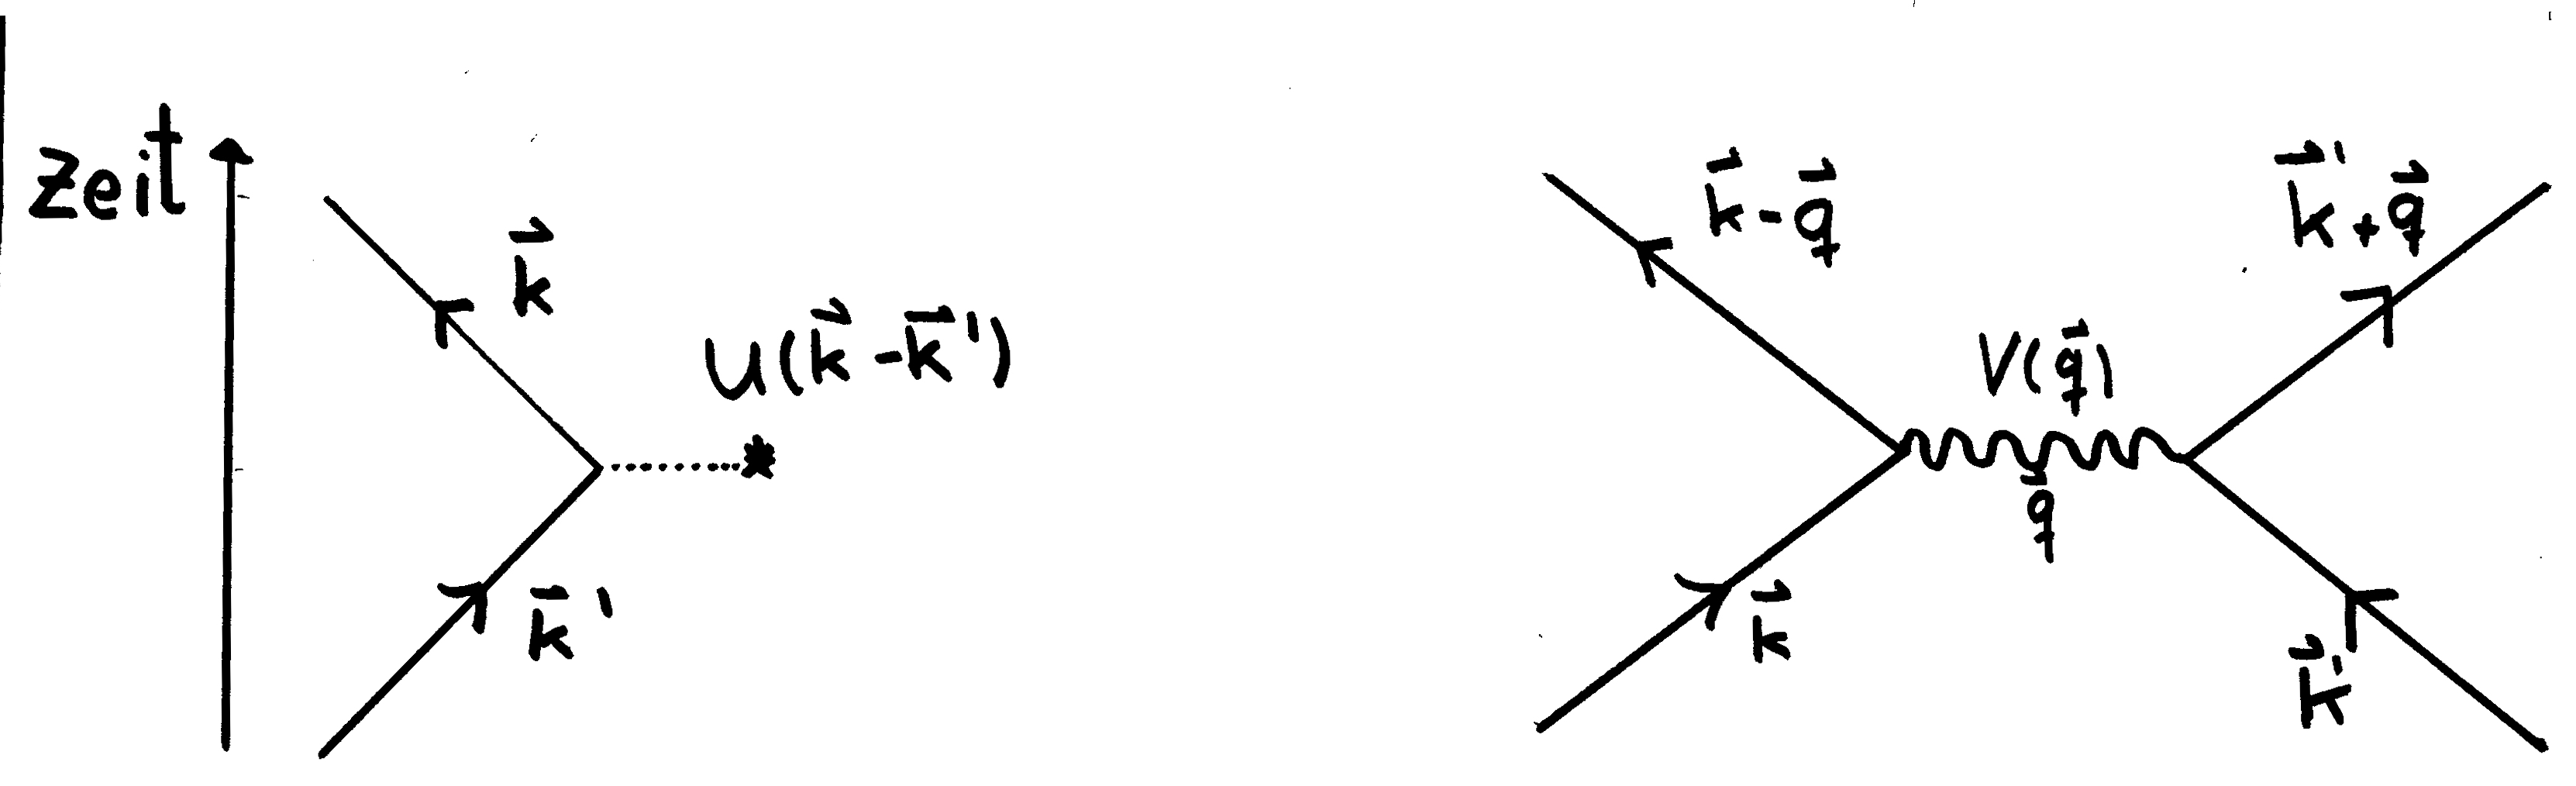
\includegraphics[scale=0.10]{Figs/Pim000113.png}
\end{center}
\subsubsection{Spin}
Feldoperatoren erhalten zusätzlichen Index $\sigma$ für den Spin. Es gilt
\begin{eqnarray*}\left[ \wh\Psi_\sigma(\vec r),\wh\Psi_{\sigma '}^\dagger(\vec r\,{'})\ri]_\pm = \delta_{\sigma\sigma'} \delta(\vec r-\vec r\,{'})
\end{eqnarray*}
Einteilchenoperatoren enthalten Summen über Spin. Zum Beispiel
\begin{eqnarray*}
\hat n (\vec r) = \sum_\sigma \wh\Psi^\dagger_{\sigma}(\vec r) \wh\Psi_\sigma (\vec r) = \sum_\sigma \hat n_\sigma (\vec r)
\end{eqnarray*}
Hamiltonoperator
\begin{eqnarray*}
\wh \ham \g \sum_\sigma \int \mathrm{d}^3r \wh\Psi_\sigma^\dagger(\vec r) \left( -\frac{\hbar^2 \Delta}{2m} + U(\vec r)\ri) \wh\Psi_\sigma(\vec r)\\
&{}&\quad + \sum_{\sigma,\sigma'} \int \mathrm{d}^3r \mathrm{d}^3r'\ \wh\Psi_\sigma^\dagger(\vec r)\wh\Psi_{\sigma'}^\dagger(\vec r\,{'}) V(\vec r, \vec r\,{'}) \wh\Psi_{\sigma'}(\vec r\,{'}) \wh\Psi_{\sigma}(\vec r)
\end{eqnarray*}
{Bemerkung:}\\
Die Wechselwirkung ist unterschiedlich zwischen Teilchen mit gleichem und ungleichem Spin.\\ \\
\underline{Spindichteoperator}
\begin{eqnarray*}
\vec S(\vec r) = \sum \limits_\alpha \delta(\vec r-\vec r\,{'}_\alpha) \vec s_\alpha
\end{eqnarray*}
Für Spin-$\frac 1 2$ Teilchen$\qquad S = \frac \hbar 2 (\sigma_x,\sigma_y,\sigma_z)$\\
In 2. Quantisierung
\begin{eqnarray*} \vec S(\vec r) = \frac \hbar 2  \sum_{\sigma \sigma'} \wh\Psi_\sigma^\dagger (\vec r ) \vec \sigma_{\sigma \sigma'}\wh\Psi_{\sigma'}(\vec r)
\end{eqnarray*}
Gesamtspin:
\begin{eqnarray*}
\vec S = \int \mathrm{d}^3r \ \vec s(\vec r)\end{eqnarray*}
Erfüllt Drehimpulsalgebra
\begin{eqnarray*}
\left [ S_i,S_j\ri] = i\hbar \varepsilon_{ijk}S_k
\end{eqnarray*}


